\documentclass{thesisclass}
% Based on thesisclass.cls of Timo Rohrberg, 2009
% ----------------------------------------------------------------
% Thesis - Main document
% ----------------------------------------------------------------

\usepackage{caption}
\usepackage{blkarray}
\usepackage{framed}
\usepackage[linesnumbered,ruled]{algorithm2e}
\usepackage{graphbox}
\usepackage{multicol}
\usepackage{minted}
\usepackage{multicol}
\usepackage{colortbl}
\usepackage{wrapfig}
\usepackage{hyperref}
\usepackage{cleveref}
\usepackage{todonotes}
\usepackage{multirow}
\usepackage{multirow}
\usepackage{booktabs}
\usepackage{environ}
\usepackage{tabularx}
\usepackage{tikz}
\usepackage[acronym,nomain]{glossaries}

%% ---------------------------------
%% | Information about the thesis  |
%% ---------------------------------

\newcommand{\myname}{Rudolf Biczok}
\newcommand{\mytitle}{Integration of internal and external gene expression and drug-perturbation data to empower novel immune therapies against Parkinson’s Disease}
\newcommand{\myinstitute}{Institute of Theoretical Computer Science}

\newcommand{\reviewerone}{Prof. Dr. Alexandros Stamatakis}
\newcommand{\reviewertwo}{Prof. Dr. Ralf Reussner}
\newcommand{\advisor}{Dr. Jitao David Zhang}

\newcommand{\timestart}{1st August 2018}
\newcommand{\timeend}{31st January 2019}

%% -------------------------------
%% |  Information for PDF file   |
%% -------------------------------

\hypersetup{
	pdfauthor={\myname},
	pdftitle={\mytitle},
	pdfsubject={Bioinformatics},
	pdfkeywords={Drug Discovery, Bioinformatics, Data Mining}
}

%% ---------------------------------
%% | Commands                      |
%% ---------------------------------

\newtheorem{definition}{Definition} \numberwithin{definition}{chapter}
\newtheorem{theorem}[definition]{Theorem}
\newtheorem{lemma}[definition]{Lemma}
\newtheorem{corollary}[definition]{Corollary}
\newtheorem{conjecture}[definition]{Conjecture}

\newcolumntype{C}{>{\centering\arraybackslash}X}

%% TODO : Is this ever used?
\NewEnviron{myTable}[4]{%
	\vspace{5px}%
	\centering%
	\rowcolors{2}{black!25}{white}%
	\captionsetup{type=table}
	\begin{tabular}{|#2|}%
		\arrayrulecolor{black}%
		\hline%
		\BODY
		\hline%
	\end{tabular}%
	\vspace{-6px}%
	\captionof{table}[#3]{#3#1} \label{#4}%
	\vspace{5px}
}

\NewEnviron{centeredFigure}[1][]{%
	\begin{figure}[#1]
		\centering
		\BODY
	\end{figure}	
}

\newcommand*\tikzCircled[1]{
	\node[shape=circle,draw,inner sep=2pt, fill=black] (char) {
		\textcolor{white}{#1}
	}
}

\newcommand*\circled[1]{
	\tikz[baseline=(char.base)]{
		\tikzCircled{#1};
	}
}

\newcommand{\thc}[1]{\textbf{\textcolor{white}{#1}}}

\newcommand{\myHeaderCell}[1]{\cellcolor{black}\thc{#1}}

\newcommand{\myMultiLineCell}[2][c]{%
	\begin{tabular}{@{}#1@{}}#2\end{tabular}%
}

\newcommand{\cbrac}[1]{\lbrace #1\rbrace}

%% --------------------------------
%% | Settings for word separation |
%% --------------------------------
% Help for separation:
% In german package the following hints are additionally available:
% "- = Additional separation
% "| = Suppress ligation and possible separation (e.g. Schaf"|fell)
% "~ = Hyphenation without separation (e.g. bergauf und "~ab)
% "= = Hyphenation with separation before and after
% "" = Separation without a hyphenation (e.g. und/""oder)

% Describe separation hints here:
\hyphenation{
% Pro-to-koll-in-stan-zen
% Ma-na-ge-ment  Netz-werk-ele-men-ten
% Netz-werk Netz-werk-re-ser-vie-rung
% Netz-werk-adap-ter Fein-ju-stier-ung
% Da-ten-strom-spe-zi-fi-ka-tion Pa-ket-rumpf
% Kon-troll-in-stanz
}

%Break links in URLs
\def\UrlBreaks{\do\/\do-}


%% ------------------------
%% |    Including files   |
%% ------------------------
% Only files listed here will be included!
% Userful command for partially translating the document (for bug-fixing e.g.)
\includeonly{
titlepage,
chapters/motivation,
chapters/introduction,
chapters/materials,
chapters/results,
chapters/conclusion,
chapters/appendix
}

% Generate the glossary
\makeglossaries

\makeatletter
\renewcommand\listoffigures{%
	\@starttoc{lof}%
}
\renewcommand\listoftables{%
	\@starttoc{lot}%
}
\makeatother

%%%%%%%%%%%%%%%%%%%%%%%%%%%%%%%%%
%% Here, main documents begins %%
%%%%%%%%%%%%%%%%%%%%%%%%%%%%%%%%%
\begin{document}

% Remove the following line for German text
\selectlanguage{english}

\frontmatter
\pagenumbering{roman}
%% titlepage.tex
%%

% coordinates for the bg shape on the titlepage
\newcommand{\diameter}{7}
\newcommand{\xone}{-15}
\newcommand{\xtwo}{160}
\newcommand{\yone}{15}
\newcommand{\ytwo}{-253}

\begin{titlepage}
% bg shape
\begin{tikzpicture}[overlay]
\draw[color=gray]  
 		 (\xone mm, \yone mm)
  -- (\xtwo mm, \yone mm)
 arc (90:0:\diameter mm) 
  -- (\xtwo mm + \diameter mm , \ytwo mm) 
	-- (\xone mm + \diameter mm , \ytwo mm)
 arc (270:180:\diameter mm)
	-- (\xone mm, \yone mm);
\end{tikzpicture}
	\begin{textblock}{10}[0,0](4,2.5)
		
\includegraphics[width=.3\textwidth]{logos/KITLogo.pdf}
	\end{textblock}
        %\begin{textblock}{10}[0,0](14.5,2.45)
		%
\includegraphics[width=.15\textwidth]{logos/algoLogo.pdf}
	%\end{textblock}
	\changefont{phv}{m}{n}	% helvetica	
	\vspace*{3.75cm}
	\begin{center}
		\Huge{\mytitle}
		\vspace*{2.25cm}\\
		\Large{
			\iflanguage{english}{Master Thesis of}			
												  {Masterarbeit\\von}
		}\\
		\vspace*{1cm}
		\huge{\myname}\\
		\vspace*{1cm}
		\Large{
			\iflanguage{english}{At the Department of Informatics}			
													{An der Fakult\"at f\"ur Informatik}
			\\
			\myinstitute
		}
	\end{center}
	\vspace*{1cm}
\Large{
\begin{center}
\begin{tabular}[ht]{l c l}
  % Gutachter sind die Professoren, die die Arbeit bewerten. 
  \iflanguage{english}{Reviewer}{Erstgutachter}: & \hfill & \reviewerone\\
  \iflanguage{english}{}{Zweitgutachter:} & \hfill & \reviewertwo\\
  \iflanguage{english}{Advisor}{Betreuender Mitarbeiter}: & \hfill & \advisor\\
  %\iflanguage{english}{}{} & \hfill & \advisortwo\\
  % Der zweite betreuende Mitarbeiter kann weggelassen werden. 
\end{tabular}
\end{center}
}


\vspace{2cm}
\begin{center}
\large{\iflanguage{english}{Time Period}{Bearbeitungszeit}: \ \timestart{} \ -- \ \timeend}
\end{center}


\begin{textblock}{10}[0,0](4,16.8)
\tiny{ 
	\iflanguage{english}
		{KIT -- University of the State of Baden-Wuerttemberg and National Laboratory of the Helmholtz Association}
		{KIT -- Universit�t des Landes Baden-W�rttemberg und nationales Forschungszentrum der Helmholtz-Gesellschaft}
}
\end{textblock}

\begin{textblock}{10}[0,0](14,16.75)
\large{
	\textbf{www.kit.edu} 
}
\end{textblock}

\end{titlepage}

\blankpage

%% -------------------------------
%% |   Statement of Authorship   |
%% -------------------------------

\thispagestyle{plain}

\vspace*{\fill}

\centerline{\textbf Statement of Authorship}

\vspace{0.25cm}

I hereby declare that this document has been composed by myself and describes my own work, unless otherwise acknowledged in the text.

\vspace{2.5cm}

\hspace{0.25cm} Heidelberg, 31st January 2019

\vspace{2cm}

\blankpage

%% -------------------
%% |   Abstract      |
%% -------------------

\thispagestyle{plain}

\begin{addmargin}{0.5cm}

\centerline{\textbf Abstract}

The primary objective of gene set enrichment analysis is to annotate genes of interest with a-priory knowledge in the form of curated gene sets. The problem in this method lies in the large number of reported gene sets and their varying information content. Previous publications suggest to use unsupervised learning methods like hierarchical clustering or self-organized maps to increase interpretability, but there is no metric to assess the quality of these clustering methods or the difference between gene sets itself. We therefore evaluated statistical methods (minkowski, jaccard, kappa-statistic), tree-based methods (gene ontology), network-based methods (shortest path in protein-protein networks), and method based on natural language processing for their capability to measure a biologically plausible distance between gene sets. We used pathway trees from Reactome and a curated tree of immune cell types with corresponding gene sets to benchmark these distance methods. \todo{TODO what is the conclusion?}

\vskip 2cm

\centerline{\textbf Deutsche Zusammenfassung}

%Kurze Inhaltsangabe auf deutsch.

\todo{Make german summary at the very end}

\vskip 2cm

\newpage

\centerline{\textbf Acknowledgements}

First and foremost I want to thank the two most valuable point of information Prof Dr. Alexandros Stamatakis and Dr. Jitao David Zhang. The open minded nature of Prof. Stamatakis made this research collaboration possible and his leading expertise in computational bioinformatics tremendously helped us to keep this master thesis in an academic format. Dr. Zhang also proved his courage and passion in academia by entrusting a theoretical biology research project to an computer science student. His knowledge as principle bioinformatician / biostatistician in an industrial and academic research environment complemented the methodical / computer science expertise of Stamatakis and me beyond expectations.

I send my greetings and thankfulness to Prof. Dr. Ralf H. Reussner, who did not hesitate to take the responsibility as second reviewer. I was a former participant in a two-term research project under the supervision of Prof. Reussner where he demonstrated a high level of methodical knowledge in the engineering aspect of computer science. 

In addition, I want to highlight the support from Gregor Sturm, Sarah Lutteropp, and Lucas Czech\todo{Will lucas be a Dr with the end of this thesis?}. Gregor Sturm is a former master thesis student of Dr. Zhang who shared the curated tree of immune cell types with their respective marker genes. He also eagerly helped me to extract  all necessary information from his publicly available code repository to save time on my side. Sarah Lutteropp is a PhD student of Prof. Stamatakis and shared her knowledge about methods and limitations in distance-based (phylogenetic) tree inference algorithms. Lucas Czech is also a PhD student under supervision of Prof. Stamatakis and provided me with an implementation skeleton for creating unsupervised clustering algorithms similar to $k$-means in C++.

Although I wish to thank every person in my live who inspired me, helped me, or even influenced my belief system, I must restrict myself to the following group of people that deserve a special place in this section: All members of the HITS Exelixis Lab (Prof. Dr. Alexandros Stamatakis, Dr. Alexey Kozlov, Lucas Czech, Sarah Lutteropp, Pierre Barbera, Benoit Morel, and Ben Bettisworth) and ROCHE BEDA group. Every single member treated me like an equal researcher.

I send my finally thanks and greetings to my parents, who are the only person on earth able to restrain my evil mind and my sister, who happened to be the younger sibling and by extension forced me to be a good role model.

\end{addmargin}

\blankpage

%% -------------------
%% |   Directories   |
%% -------------------

\tableofcontents
\listoftodos
\blankpage

%% -----------------
%% |   Main part   |
%% -----------------

\mainmatter
\pagenumbering{arabic}

%% ==============================
\chapter{Motivation}
\label{ch:motivation}
%% ==============================

\newacronym{rna}{RNA}{Ribonucleic Acid}
\newacronym{dna}{DNA}{Deoxyribonucleic Acid}
\newacronym{ppi}{PPI}{Protein Protein Interactions}

Molecular biology is the aspect of life science thats investigates biological processes on a cellular and molecular level. Biologists in this area seek answers for questions like: ``What is the structural and functional difference between neuron cells compared to other cell types in mammal species?'', ``What influence has chemical compound A when introduced to cell line C?'', or ``Is the cell line derived by following lab protocol A different from the cell line of protocol B?''.
%\begin{wrapfigure}{r}{0.4\textwidth}
%	\centering
%	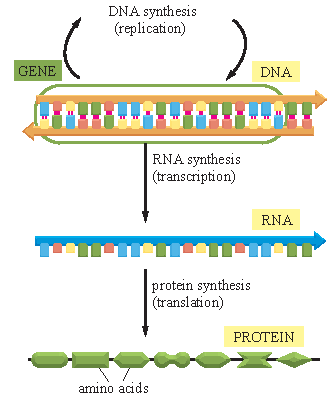
\includegraphics{figures/motivation/central_dogma.pdf}
%	\caption{Central dogma of molecular biology~\cite{citeulike:691434}}
%	\label{fig:central_docma}
%\end{wrapfigure}
%The biggest problem in answering this questions lies within the black-box nature of every living cell. We know that genes play an important role in determine the structure and basic behavior (also known as morphology) of every organism~\cite{citeulike:691434}. Ongoing research also reveals the functionalities behind each gene ofna n or    
The common procedure to research these questions is to conduct wet lab experiments on prepared cell cultures followed by a computer-assistant gene expression analysis. 
Gene expression is the fundamental biological process of every organism that describes the transcription of \acrfull{rna} from \acrfull{dna} and the translation from \acrshort{rna} to proteins~\cite{citeulike:691434}. 
Collecting and analyzing the gene expression level of every gene inside an organism allows us to identify differentially expressed genes that cause morphological differences between cell groups or cell types~\cite{doi:10.1093/bioinformatics/btp616}. To the end, bioinformaticians use public databases of gene sets to see which known cell components or biological processes are reflected by the previously inferred list of differential expressed genes. 
Every gene set represents discovered knowledge in form of name, description and involved genes of a particular biological process. 
Ideally, the entire procedure results in a list of gene sets that uniquely explain the effects of the original wet lab experiment~\cite{doi:10.1093/nar/gks461} (see \cref{sec:gene_expression} for further information about gene expression analysis).

In reality, however, the information gain from reported gene sets is unsatisfying, because 
1) gene sets from even the same database source tend to have a high gene overlap, 
2) gene sets from publicly available databases can have many genes (>200), and 
3) gene set information like title and description can vary in quality depending on the source.
Existing literature suggest supervised learning methods to organize gene sets into a more representative structure. The DAVID algorithm, for instance, performs agglomerative clustering over pairwise kappa statistic between gene sets~\cite{Huang2007}. The authors of this algorithm claim that it maximizes the number of pairwise \acrfull{ppi} within each gene set cluster. However, they also state that it is unclear if this optimization criterion is biologically justified. In general, there exist no gold standard to asses the biological similarity between two gene sets. Having such a gold standard the other hand would make it possible to compare gene set as elements of a metric space. It would enable researchers to benchmark and refine clustering algorithms or to discover new insights from the rapidly growing amount of gene set data.

\section{Own contribution}

We present in this thesis a systematic evaluation of different distance metrics for pairwise gene set comparisons. We implemented metrics based on 1) statistic methods, 2) gene ontology trees, 3) protein-protein interaction graph networks, and 4) natural language processing methods. For comparing the performance of each distance implementation, we extracted gene sets from data sources whose relationships are already know and preserved as rooted trees. These data sources include 2\todo{update to newest} subsets of the Reactome pathway database~\cite{doi:10.1093/nar/gki072} and a manually curated collection of marker genes for 36\todo{update to newest} human immune cell types~\cite{Sturm463828}. We bundled all distances implementations, data preprocessing, and analysis scripts into a Python package that can be readily extended or included into other algorithms.

Besides gene set analysis, we also spend a significant amount of time building a gen expression analysis framework based on Python. It utilizes a client-server architecture with3 different front-ends for executing and persisting new gene expression experiments (see \cref{sec:roger} for more information).

\section{Structure of this thesis}

The reminder of this document follows the structure of a conventional bioinformatics paper. In \cref{ch:introduction}, we will explain the anatomy of a gene expression analysis pipeline in greater details. In addition, the introduction chapter will cover basic concepts about natural language processing with Word2Vec models and the composition about biological data sources (e.g. gene ontologies, \acrshort{ppi} networks).

\Cref{ch:methods} gives more details about the algorithms behind each implemented distance metric. We will also summarize the preprocessing steps for the used evaluation data in this chapter.

In \cref{ch:results}, present benchmark results from each distance metric over the different sets of evaluation date. We will also discuss certain outcome of the results and assess the limitations of different distance metrics. \todo{Mention the key points here}

And finally, we will draw a final conclusion about our conducted experiments and we will give a future outlook about potential follow-up research in \cref{ch:results}.

%% ==============================
\chapter{Introduction}  \label{ch:introduction}
%% ==============================

%A reader of the introduction should be able to answer the following questions, although not in any depth.
%
%    What is the thesis about?
%    Why is it relevant or important?
%    What are the issues or problems?
%    What is the proposed solution or approach?
%    What can one expect in the rest of the thesis?
%
%State what the thesis is about early. Don't keep the reader guessing until the end of the introduction, or worse, the end of the thesis (don't laugh, I have read draft theses that left me wondering after reading the entire document). You should provide a brief and gentle overview of the thesis topic (or problem) to give the reader enough context  to understand the rest of the introduction. Don't overwhelm the reader with detail at the start. You will provide the details later elsewhere in the thesis. Target the level of writing at one of your peers, but not necessarily somebody working in the same area.
%
%State why the topic is important. Address the "so what?" criteria. Why are you working on the topic? Why should somebody else be interested? Your motivation should be obvious after the introduction, but not necessarily provably so at this point.
%
%State what the major issues are in solving your problem. Coherently overview the issues in enough detail to be able to understand they exist, but don't go into details yet or attempt to prove they exist. The overview should be in just enough depth to understand why you might propose the your particular solution or approach you are taking.
%
%Describe your proposed solution or position you're taking. Again, you should not go into minute details, nor should you attempt to prove your solution at this point; the remainder of the thesis will describe and substantiate your solution in detail, that's what a thesis is :-)
%
%At this point the reader will know what you're working on, why, what are the major issues, and what your proposed solution is, but usually only if he takes your word for it. You should outline what the reader should expect in the rest of the thesis. This is not just the table of contents in sentence form, it is an overview of the remainder of the thesis so the reader knows what to expect. 
%
%
%--------------------------------
%

\section{Gene expression analysis} \label{sec:gene_expression}

\newacronym{rnaseq}{RNA-Seq}{RNA sequencing}
\newacronym{scrnaseq}{scRNA-Seq}{signle cell RNA sequencing}
\newacronym{dge}{DGE}{Differential gene expression}
\newacronym{gse}{GSE}{Gene set enrichment}

Gene set enrichment is the bread and butter of every bioinformatician who tries to discover the genetic reason for morphological differences between cell lines. The basic process involves a series of wet and dry lab operations (\cref{fig:gene_expression_analysiss}).

\begin{centeredFigure}[!h]
	\resizebox{\textwidth}{!}{% <------ Don't forget this %
		\begin{tikzpicture}
			\node[inner sep=0pt] (monocyte1) at (0,0) {
				S1 \enspace 
\includegraphics[align=c, width=1.1cm]{figures/introduction/macrophage.png}
			};
			\node[inner sep=0pt] (monocyte2) at (0,-1) {
				S2 \enspace 
\includegraphics[align=c, width=1.1cm]{figures/introduction/macrophage.png}
			};
			\node[inner sep=0pt] (macrophage1) at (0,-2) {
				S3 \enspace 
\includegraphics[align=c, width=1.1cm]{figures/introduction/microglia.png} 
			};
			\node[inner sep=0pt] (macrophage2) at (0,-3) {
				S4 \enspace 
\includegraphics[align=c, width=1.1cm]{figures/introduction/microglia.png} 
			};
		
			\node[align=center] (gct) at (6,-1.6) {
				\textbf{Expression data} \\[3pt]
				\setlength\tabcolsep{3pt}
				\begin{tabular}{r|c|c|c|c}
				   	        &    S1  &      S2 & S3 & S4  \\
						\hline
					Sensor 1 &    240 &    415 & 78 & 81 \\
					Sensor 2 &      12 &       4 & 55  & 3  \\
					Sensor 3 &       0 &        0 &        0 &        0  \\
				  	\ldots & \ldots & \ldots & \ldots & \ldots 
				\end{tabular}
			};
		
			\draw [->, ultra thick] (macrophage1.north east) --
				 node [midway,above, align=center] {expression \\ measurement} 
				 node [midway,below, align=center] {microarray, \\ RNA-seq, \\ scRNA-seq, \\ \ldots}
				 (gct);
		
			\node[align=center] (dge) at (13,-1.6) {
				\textbf{DGE top table} \\[3pt]
				\setlength\arrayrulewidth{2pt}
				\setlength\tabcolsep{0pt}
				\arrayrulecolor{white}
				\begin{tabular}{r|c|c|c|c}
					& S1  & S2 & S3 & S4  \\
					\hline
					COL1A1 & \cellcolor{red} & \cellcolor{red!80} & \cellcolor{blue!50} & \cellcolor{blue!20} \\
					\hline
					PLEC & \cellcolor{red!80} & \cellcolor{red!60} & \cellcolor{blue!70} & \cellcolor{blue!50} \\
					\hline
					LOXL4 & \cellcolor{blue!50} & \cellcolor{blue!30} & \cellcolor{red!80} & \cellcolor{red!60} \\
					\ldots & \multicolumn{4}{c}{\ldots} \\
				\end{tabular}
				\arrayrulecolor{black}
			};
		
			\draw [->, ultra thick] (gct) -- 
				node [midway,above] {DGE analysis} 
				node [midway,below, align=center] (dgedesc) {edgeR, \\ DGEseq, \\ limma, \\ \ldots} (dge);
		
			\node[align=left, draw=black, ultra thick, inner sep=3pt,] (gse) at (20.5,-1.6) {
				\textbf{Gene set top table} \\[1em]
				\textit{1. Anchoring fibril formation} \\
				$\left\lbrace COL1A1, COL1A2, \ldots \right\rbrace$ \\[0.5em]
				
				\textit{2. Formation of collagen fibres} \\
				$\left\lbrace LAMA3, LOXL4, \ldots \right\rbrace$ \\[0.5em]
				
				\textit{3. Hemidesmosome formation} \\
				$\left\lbrace PLEC, LAMB3, \ldots \right\rbrace$
			};
		
			\draw [->, ultra thick] (dge) -- 
				node [midway,above] {GSE analysis} 
				node [midway,below, align=center] {CAMERA, \\ \ldots} (gse);
		
			\node[align=right] (fanno) at (5,-6) {
				\textbf{Feature annotation} \\[3pt]
				\setlength\tabcolsep{3pt}s
				\begin{tabular}{r|c|c|c}
					& Symbol & Name& \ldots \\
					\hline
					Sensor 1 & COL1A1 & Collagen type I alpha 1 chain  & \multirow{4}{*}{\vdots} \\
					Sensor 2 & COL1A2 &  Collagen type I alpha 2 chain &  \\
					Sensor 3 & LAMA3 &  Laminin Subunit Alpha 3  &  \\
					\ldots & \ldots & \ldots & \\
				\end{tabular}
			};
		
			\node[align=left] (sanno) at (14.5,-6) {
				\textbf{Sample annotation} \\[3pt]
				\setlength\tabcolsep{3pt}
				\begin{tabular}{r|c|c|c}
					& Cell type & Replication & \ldots  \\
					\hline
					S1 & Macrophage & 1 & \multirow{4}{*}{\vdots} \\
					S2 & Macrophage &  2 &  \\
					S3 & Microglia & 1 & \\
					S4 & Microglia & 2 & \\
				\end{tabular}
			};
		
			\draw [->, ultra thick] (fanno) -- (dgedesc);
		
			\draw [->, ultra thick] (sanno) -- (dgedesc);
		
			\node at (0,1) {\circled{1}};
			\node at (6,1) {\circled{2}};
			\node at (13,1) {\circled{3}};
			\node at (21,1) {\circled{4}};
			
			\node at (5,-4) {\circled{5}};
			\node at (14,-4) {\circled{6}};
		
		\end{tikzpicture}% <------ Don't forget this %
	}
		
	\caption{Gene expression analysis work flow}
	\label{fig:gene_expression_analysiss}
\end{centeredFigure}

At first \circled{1}, a biologist prepares at least two groups of cell lines (generally called samples). The grouping depends on the desired comparison a researcher wants to study, like different immune cell types (e.g. macrophages vs microglia cells~\cite{10.3389/fncel.2013.00045}), healthy cells vs. tumor cells, or perturbed vs. non-perturbed cells. By perturbation we mean any type of cell modification (gene knock-out) or manipulation of the cell environment (e.g. adding drug compounds). It is common practice to cultivate more than one cell line under the same experimental condition (aka. technical replicates) to ensure reproducibility.

The next task describes the generation of gene expression profiles \circled{2}. This involves fixing the cells,  dissolving their membrane, and extracting all \acrshort{rna} fragments. Different methods exist to quantify the \acrshort{rna} concentration per gene and by extension the expression levels. The most frequently used methods are microarray assays, \acrfull{rnaseq}~\cite{citeulike:691434}, and \acrfull{scrnaseq}~\cite{Eberwine2013}. Each method requires different laboratory tasks and computational preprocessing algorithm. The end result of this stage is a table that shows the expression levels for every gene in every sample. The actual meaning of the value can differ depending on the used preprocessing technique. In can, for instance, stand for the total number of \acrshort{rna} fragments counted per gene when using \acrshort{rnaseq}.

After obtaining the raw data, a bioinformatician use linear models to detect genes that are differentially expressed between sample groups \circled{3}. For instance, a widely used software package called edgeR models the entire gene expression experiment as negative binomial distribution to control gene-wise dispersion~\cite{doi:10.1093/bioinformatics/btp616}. The package edgeR uses a variant of the Fisher's exact test to detect \acrfull{dge}. Other packages like limma~\cite{doi:10.1093/nar/gkv007} or DGEseq~\cite{doi:10.1093/bioinformatics/btp612} are flavored depending on the number of technical replicates or used expression measurement technique. 

Experience tells us that genes reported from \acrshort{dge} analysis alone give to view information behind the actual biological phenomena. A single gene can be involved in multiple, partially unknown biological processes or is just an artifact from prior \acrshort{dge} analysis. \acrfull{gse} algorithms try to overcome this issue by using statistical methods and external information about biological processes. One prominent example is implemented in the software package CAMERA~\cite{Wu2012}, which uses competitive gene set tests. The idea behind this competitive tests is to compare every genes inside a gene set relatively to all other genes measured in the experiment. CAMERA in particular uses a modified two-sided $t$-tests capable of detecting inter-gene correlations. The result of this step is a high score \circled{4} of gene sets reflected by the prior list of differentially expressed genes. The content of gene sets used for the \acrshort{gse} is arbitrary and the depends on what sources the bioinformatician choses for analysis. Gene sets from MSigDB~\cite{doi:10.1093/bioinformatics/btr260}, for instance, contains genes that characterize a specific cell type or cell condition. The database Reactome~\cite{doi:10.1093/nar/gki072} on the other hand offers gene sets containing these genes that are part of a particular biological process (aka. pathway).

It is important to note the entire process relies on the existence of feature annotation data \circled{5} and sample annotation data \circled{6}. The feature annotation gives additional information about the measured genes (e.g. name and description of the actual gene that is associated with a particular sensor slot). The sample annotation hold information about origin, and preparation steps for each analyzed cell sample (e.g. cell type, tissue origin, used chemicals).

\section{Pathway \& protein-protein interaction networks}

We can describe every reaction inside or outside a cell as network of protein interactions with organic chemicals, \acrshort{rna}, \acrshort{dna}, or other proteins. \Cref{fig:pathway} illustrates an excerpt of such an interaction network during the mitotic cell cycle.

\begin{centeredFigure}[!h]
	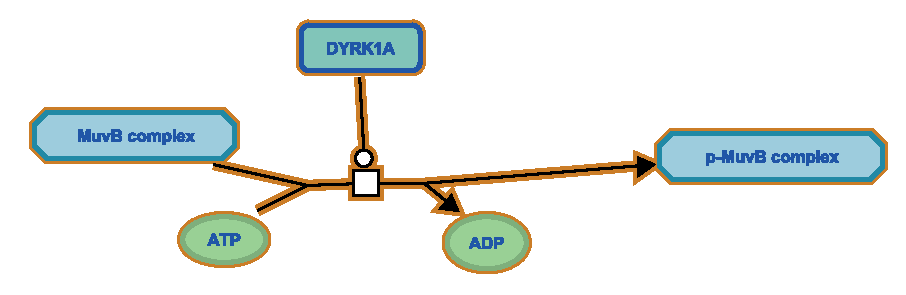
\includegraphics[scale=0.8]{figures/introduction/pathway.pdf}
	\caption{Expert of the mitotic cell cycle.  The rectangular boxes and boxes with octagon shape represent proteins. The green nodes represent other organic compounds. The entire pathway involves over different 400 proteins}
	\label{fig:pathway}
\end{centeredFigure}

Public databases like BioGRID~\cite{doi:10.1093/nar/gkw1102} offer a collection of known protein-protein interaction as annotated edge-list. Each edge represents the interaction between one protein with another and hold information about author, detection method, and interaction type. We can use these data sources to compare gene sets in a graph-based representation. It is important to note that not all protein-protein interactions are necessarily part of an actual biological process. This applies for these  protein-protein interactions that researchers discovered outside a cell through regular chemical reaction assay. We use the term pathway to distinguish comprehensive protein-protein interaction networks provided by BioGRID with networks that are know to exist in living cells. \todo{reference for BioGRID}

\section{Gene ontology}

\newacronym{go}{GO}{Gene Ontology}

The \acrfull{go} maintained by the gene ontology consortium~\cite{Ashburner2000,doi:10.1093/nar/gkw1108} is a collection fo controlled vocabulary (aka. \acrshort{go} terms). Every term has is unique identifier (e.g. GO:0030234) and is associated in one of three categories: 1) biological process (e.g. wound healing, epithelial cell proliferation), 2) cellular component (cytoplasm, organelle part), and 3) molecular function (e.g. catalytic activity, enzyme regulator activity).

\begin{centeredFigure}[!h]
	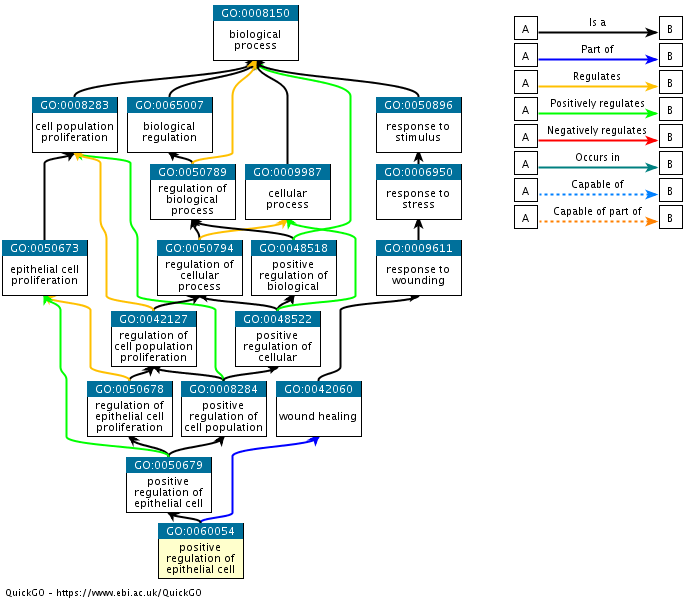
\includegraphics[scale=0.4]{figures/introduction/go.png}
	\caption{Excerpt of the gene ontology}
	\label{fig:go}
\end{centeredFigure}

\acrshort{go} terms can have 8 different type of relationships between each other, as seen in \cref{fig:go}. If we only consider the ``is a'' relationships, all \acrshort{go} term of the same category resemble a rooted tree structure. In addition, the gene ontology consortium maintains a mapping between \cref{fig:go} terms and gene identifier, where each \cref{fig:go} term is associated with multiple gene identifiers. 

Researcher can use the gene ontology for \acrshort{gse} analysis, where the reported ``gene sets'' are \acrshort{go} terms~\cite{doi:10.1093/bioinformatics/btl140}.  Additionally, algorithms exist to define an arithmetic similarity measurement for \acrshort{go} terms~\cite{doi:10.1093/bioinformatics/btq064}.

\section{Natural language processing}

\newacronym{nlp}{NLP}{Natural Language Processing}
\newacronym{bow}{BOW}{Bag Of Words}
\newacronym{wmd}{WMD}{Word Mover Distance}

According to Pyysalo et al. \cite{Pyysalo:2013b}, publication databases like the PubMed Central (PMC) contain over 700,000 full-text articles with valuable information about biological processes. \acrfull{nlp} techniques like word embeddings opens the opportunity to detect linguistic relationships within unstructured text as it is found in literature databases.

\subsection{Word embedding}

Word embeddings are a class of machine learning models that learn feature vectors from a large set of arbitrary text (aka. text corpus). These feature vectors can be used to project words in a vector space while preserving their semantic similarities. For instance, assume two genes which are part of the same pathway. Then it is likely that the name of the genes appear relatively close to each other in multiple publication. Word embeddings reflect the text distances between the gene names to the feature vector space. Mature examples of world embedding are word2vec techniques, which use feedforward neural as supervised learning method networks~\cite{journals/corr/abs-1301-3781}. 
%\Cref{fig:w2v} shows the two variants of the word2vec model. 

%\begin{centeredFigure}[!h]
%	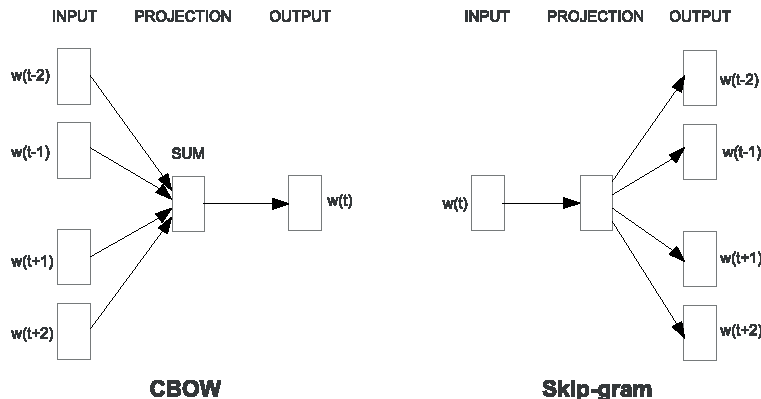
\includegraphics{figures/introduction/word2vec.pdf}
%	\caption{The two variants of the word2vec learning method \cite{journals/corr/abs-1301-3781}}
%	\label{fig:w2v}
%\end{centeredFigure}

\subsection{Document queries}

Inside a vector space, we can use mathematical functions like the euclidean distance or the cosine distance to measure the similarity between single word. However, gene sets consists of multiple genes and can carry additional information like a description or \acrshort{go} terms. One method to compare two sets of words (aka. documents) with each other is word averaging, where the pairwise sum or average of all word vectors build a representation of the document. Kusner et al. claims, however, that ignoring individual word distances could poor comparability between documents that have few words in commin~\cite{Kusner:2015:WED:3045118.3045221}. Other solutions to this problem would be the use of alternative vector representations (e.g. \acrfull{bow}) or more sophisticated distances based on the conventional word vectors (e.g. \acrfull{wmd})~\cite{Kusner:2015:WED:3045118.3045221}. 

%% ==============================
\chapter{Materials and methods} \label{ch:methods}
%% ==============================

\section{Reference data}

\subsection{Reactome reference tree}

\subsection{Immune cell differentiation hierarchy}

\section{Distance measurements}

\subsection{Mathematical measurements}

\subsection{Network-based measurements}

%Studying these networks and identifying their unique functions in the cell live-cycle is a time-consuming task and involves requires laboratory techniques like gene-editing, micro fluorescence, and sequencing. 

Shortest path problem:
Not Robust (show example)
* k-shortest path better, but also not that Robust
* Robust shortest path problem is NP-complete and therefore prohibited


Variances:
Average over pairwise node paths violates d(x,y) = 0 <=> x=y condition
Mean over Min of 

\subsection{Word2vec models \& measurements}

%  NLP Word Processing:
%* split (\s,",",(,),<br>), lowercase
%* Worder len > 1
%* filter stopwords
%* filter what is not in vocabulary of trained data



%\section{Gene Expression Analysis}
%
%The most recurring task in pharmaceutical research \& early development is the gene expression analysis on a given date source. 
%
%\subsection{Methods for differential gene expression inferrence}
%
%Name | Strategy | Prefered Input Data
%-----|------------|--------------------
%[edgeR](http://doi.org/10.1093/bioinformatics/btp616) | Negative binomial distribution + Trimmed Mean of M values (TMM) Normalization | RNAseq
%[DEseq](https://doi.org/10.1186/s13059-014-0550-8) | Negative binomial distribution + scaling factor normalization procedure | RNAseq
%[limma](https://doi.org/10.1093/nar/gkv007) | Linear Modeling + voom transformation of counts (vor RNAseq) | RNAseq \& microarray
%
%The "rule of thumb" is to use limma for microarray data and edgeR for RNAseq data. DEseq is used to verify that a hypothesis based on edgeR results can also be derived from DEseq results (since edgeR is known to report more false positives).
%
%\subsection{Methods for batch-effect correction in meta-analysis}
%
%We use ComBat, SVA, and BioQC. Here we will probably have to compare different methods and reach a conclusion.
%
%\subsection{Methods for gene-set/pathway enrichment analysis}
%
%We use CAMERA, BioQC, and Fisher's exact test.
%Previously we found out that CAMERA and BioQC will lead to false negatives when many genes are differentially expressed, while Fisher's exact test will not (not published). We can verify this and make a meta-method to accommodate different scenarios.
%
%\section{ROGER}
%
%\subsection{ROGER Database}
%
%* **Annotations**
%* Gene Annotation (consumes biomart)
%* GeneAnnotation: Ensemble \& NCBI gen IDs. ROGER-internal GeneIndex, Gen meta data
%* Orthologs: Mapping between orthologous genes between different species
%* TranscriptioAnnotation: Ensemble Transcription ID and meta data
%* TranscriptRefSeq: NCBI Transcription ID and meta data
%* Genesets (consumes mongodb/json \& gmt)
%* DefaultGenesets: Available gen set data
%* DefaultGenesetCategory: For gen set categorization
%* DefaultGenesets2gene: Mapping of gen set data to gen annotations
%* **Input**
%* Datasets: Raw expression data
%* Phenodata
%* Designs: Relevant Feature matrix
%* Contrasts: Contrast matrix
%* **Methods \& Results**
%* GSEmethods: Used Gen enrichment method (e.g. CAMERA)
%* GSEtables: Gen enrichment results
%* DGEmethods: Used Differential Gen Expression inference method (e.g.  edgeR, limma)
%* DGEmodels: Used DGE model based on Desing and Cntrast information
%* DGEtables: Results from DEG inference
%
%\subsection{Annotation Problems}
%
%* Have to support both Ensembl and NCBI IDs
%* Ensembl has many unconsistent / deprecated data: Some Gene Symbols apper in multiple EnsembleGeneIds, 
%* Possible fix: pick the "most accurate on" (e.g. does it have a proper chromosone? Number of Transcripts etc.)
%
%% ![ROGER Schema](roger/old_schema.png)
%
%\subsection{RESTful APIs for scientific R pipelines}
%
%* [rplumber](https://www.rplumber.io/)
%* Fastest way to deploy REST services
%* Very low-level: No load balancing, no authentication, task management, ...
%* [OpenCPU](https://www.opencpu.org)
%* Load balancing
%* Lightwing WEB API basedn on JavaScript
%* No build-in support for [long running jobs]
%(https://github.com/opencpu/opencpu/issues/141)
%* No build-in task management
%* [Flask](http://flask.pocoo.org)
%* Python equivalent to OpenCPU
%* Established in the department
%* Requires wapper functions between python <-> R
%* No build-in task management
%
%\section{Differential Gene Expression}
%
%Lets assume we have a study consisting of a set of samples $D = \cbrac{A, B, C, D, E, F}$. Samples $A$ and $B$ are from macrophage cells, $C$ and $D$ are from microglia cells, and $E$ and $F$ are from monocyte cells. 
%
%Then we have basically two ground ways to model the experiments:
%
%\begin{lrbox}{\saveBoxOne}
%	\mintinline{R}{model.matrix(~CellType)} 
%\end{lrbox}
%
%\begin{lrbox}{\saveBoxTwo}
%	\mintinline{R}{model.matrix(~0+CellType)}
%\end{lrbox}
%
%\begin{lrbox}{\saveBoxThree}
%\begin{minipage}{5cm}
%	\[
%		\begin{blockarray}{cccc}
%			& \mu & \text{\rotatebox{90}{micro}} & \text{\rotatebox{90}{mono}} &  \\
%			\begin{block}{c(ccc)}
%				A & 1 & 0 & 0  \\
%				B & 1 & 0 & 0  \\
%				C & 1 & 1 & 0  \\
%				D & 1 & 1 & 0  \\
%				E & 1 & 0 & 1  \\
%				F & 1 & 0 & 1  \\
%			\end{block}
%		\end{blockarray}
%	\]
%\end{minipage}
%\end{lrbox}
%
%\begin{lrbox}{\saveBoxFour}
%\begin{minipage}{5cm}
%	\[
%		\begin{blockarray}{cccc}
%			& \text{\rotatebox{90}{macro}} & \text{\rotatebox{90}{micro}} & \text{\rotatebox{90}{mono}} &  \\
%			\begin{block}{c(ccc)}
%				A & 1 & 0 & 0  \\
%				B & 1 & 0 & 0  \\
%				C & 0 & 1 & 0  \\
%				D & 0 & 1 & 0  \\
%				E & 0 & 0 & 1  \\
%				F & 0 & 0 & 1  \\
%			\end{block}
%		\end{blockarray}
%	\]
%\end{minipage}
%\end{lrbox}
%
%\begin{lrbox}{\saveBoxFive}
%	\begin{minipage}{5.3cm}
%		\[ y \thicksim \mu + \beta_{\text{micro}} x_{\text{micro}} + \beta_{\text{mono}} x_{\text{mono}}\] 
%	\end{minipage}
%\end{lrbox}
%
%\begin{lrbox}{\saveBoxSix}
%	\begin{minipage}{5.3cm}
%		\[ \begin{split}
%		y \thicksim \ & \beta_{\text{macro}} x_{\text{macro}} + \beta_{\text{micro}} x_{\text{micro}} \\
%		& \beta_{\text{mono}} x_{\text{mono}}
%		\end{split} \]
%	\end{minipage}
%\end{lrbox}
%
%\begin{lrbox}{\saveBoxSeven}
%			\begin{minipage}{5.3cm}
%				\[
%					\begin{blockarray}{ccc}
%						\begin{block}{c(cc)}
%						\mu          & 0 & 0 \\
%						\text{micro} & 1 & 0 \\
%						\text{mono}  & 0 & 1 \\
%						\end{block}
%					\end{blockarray}
%				\]
%		\end{minipage}
%\end{lrbox}
%
%\begin{lrbox}{\saveBoxEight}
%	\begin{minipage}{5.3cm}
%			\[
%			\begin{blockarray}{cccc}
%			\begin{block}{c(ccc)}
%			\text{macro} & -1 & -1 & 0\\
%			\text{micro} & 1 & 0 & -1 \\
%			\text{mono}  & 0 & 1 & 1 \\
%			\end{block}
%			\end{blockarray}
%			\]
%	\end{minipage}
%\end{lrbox}
%
%\begin{table}[ht]
%
%	\begin{tabularx}{\linewidth}{|lCC|}%
%		\arrayrulecolor{black}%
%		\hline
%	
%		\rowcolor{black} & \thc{1 vs Average} & \thc{1 vs 1} \\
%	
%		\circled{1} & \usebox{\saveBoxOne} & \usebox{\saveBoxTwo} \\
%		\hline%
%	
%		\circled{2} & \usebox{\saveBoxThree} & \usebox{\saveBoxFour} \\
%		
%		\circled{3} & \usebox{\saveBoxFive} 
%		& \usebox{\saveBoxSix}  \\
%
%		\circled{4} & \usebox{\saveBoxSeven} 
%		& \usebox{\saveBoxEight}  \\
%		\hline%
%		
%		\hline
%	\end{tabularx}
%
%	\caption{Overview of example experiments} \label{fig:example_experiments}
%\end{table}
%


%% ==============================
\chapter{Results \& Discussion}
\label{ch:results}
%% ==============================

\section{Ground-truth comparison}

\section{Limitations}

%% ==================
\chapter{Conclusion}
\label{ch:conclusion}
%% ==================

%Recap on your thesis. It has been a long journey if the reader has made it this far. Remind the reader what the big picture was. Briefly outline your thesis, motivation, problem, and proposed solution.

%Now the most important part, draw conclusions based on your analysis. Did your proposed solution work? What are the strong points? What are the limitations?

%Significant issues identified in the thesis, or still outstanding after the thesis, should be describe as future work.

%% ----------------
%% |   Appendix   |
%% ----------------

\cleardoublepage

\appendix

%% ==============================
\chapter{Appendix}
\label{ch:appendix}
%% ==============================


\section{ROGER - Roche Omnibus of Gene Expression Regulation} \label{sec:roger}

\subsection{State of the art}

\subsubsection{Transcriptomic data management}

\subsubsection{Differential Gene Expression Analysis}

\subsubsection{Gene Set Enrichment Analysis}

\subsection{Reimplementation}

\subsubsection{Data structures \& architecture}

\subsubsection{Visualizations \& data access}
 
\newpage 

\section{List of acronyms}
%\setglossarysection{section}
\renewcommand{\glossarysection}[2][]{}
\printglossaries

\section{List of figures}

\listoffigures

\section{List of tables}

\listoftables

\normalsize

%% --------------------
%% |   Bibliography   |
%% --------------------

\cleardoublepage
\phantomsection
\addcontentsline{toc}{chapter}{\bibname}

\iflanguage{english}
{\bibliographystyle{alpha}}
{\bibliographystyle{babalpha-fl}} % german style

\bibliography{references}

\end{document}
